\documentclass[11pt]{report}

\usepackage{graphicx}
%\usepackage[margin=0.5in]{geometry}
\usepackage{amsmath}
\usepackage{amssymb}
\usepackage{hyperref}

\title{Visual Odometry from Stereo}
\author{Alankar Kotwal -- 12D070010, Anand Kalvit -- 12D070032}

\begin{document}
\maketitle
\newpage

\section*{Introduction}
Odometry refers to the use of data from motion sensors to estimate change in position over time. One of the most reliable ways of estimation of 3-D structure using cameras is to use a calibrated stereo pair. Given the sequence of 3-D structures generated by the stereo camera, we can estimate the motion of the camera with respect to its environment as well as generate a 3-D map of the environment. This is usually referred to as visual SLAM (simultaneous localisation and mapping), which has wide applications in robotics and remote sensing. \\

\noindent We plan to implement a 6 DoF pose estimation algorithm using a calibrated stereo pair and generate a 3-D map of the environment simultaneously. We assume, for finding correspondences properly, that scene illumination doesn't change much and most of the field of view of the camera is occupied by static parts of the environment. \\

\noindent In a nutshell, our job is to figure out what the translation and rotation of the camera is between two scenes as shown below. \\ \\
\centerline{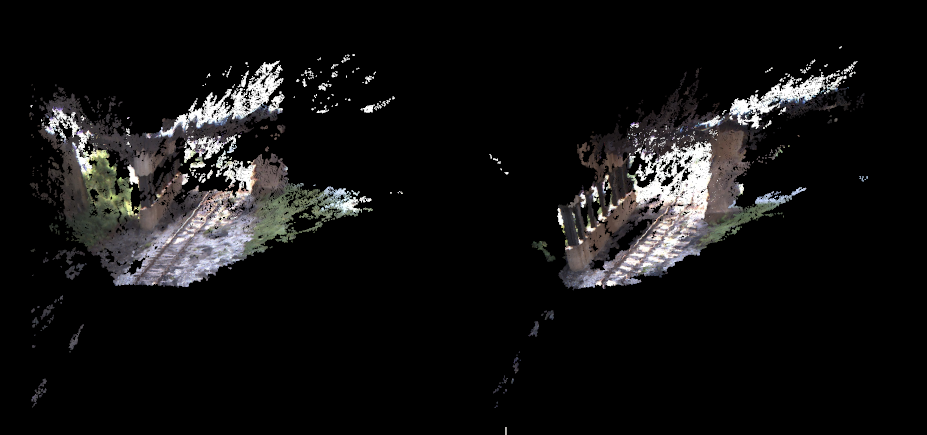
\includegraphics[scale=0.50]{pointclouds}}
\newpage

\section*{Methods We're Thinking of Using}
We will mostly use shape from stereo directly from MATLAB. \\

\noindent Once we get pointcloud information, we need to track features across pointclouds (or images) in order to estimate the motion between frames. We can use a couple of methods for this:
\begin{itemize}
\item Iterative Closest Point
\item Point Set Registration Using Gaussian Mixture Models
\item Direct Least-Squares Estimation of Pose, using point matching using feature descriptors (corner detectors or SIFT-like for images or 3D-SIFT for pointclouds).
\end{itemize}

\noindent We have not yet decided which among these will be used.

\section*{Code Details}
We will be coding in MATLAB. All code will be pushed to \url{https://www.github.com/alankarkotwal/stereo-vo}.

\section*{Datasets and Validation}
We originally thought of using data from Chandrayaan-I's Terrain Mapping Camera (which was a stereo camera) for testing purposes (since ground truth about probe position and lunar DEMs are available). We can also test our algorithm on any standard stereo image database like \url{http://vision.middlebury.edu/stereo/data} or \url{http://www.cvlibs.net/datasets/kitti/eval_stereo_flow.php?benchmark=stero}

\end{document}